\documentclass[12pt]{article}
\usepackage{amsmath}
\usepackage{polynom}
\usepackage[utf8]{inputenc}
\usepackage{pgfplots}
\pgfplotsset{width=7cm,compat=newest}
\usepackage{tcolorbox}

\title{Precalculus 12 Review}
\author{Alyssa Motas}
\date{J.L. Ilsley High School --- \today}

\begin{document}
	
	\maketitle

\section{Function Transformations}
\subsection*{1.1 - 1.3 Translations, Reflections, and Stretches}

This is the general equation when transformating an equation.

\begin{tcolorbox}
	
\begin{equation*}
y=af[b(x-h)]+k
\end{equation*}

$a$ = Vertical Stretch/Reflection on the x-axis \\
$b$ = Horizontal Stretch in the form of $\frac{1}{\text{HS}}$/Reflection on the y-axis \\
$h$ = Horizontal Translation \\
$k$ = Vertical Translation

\end{tcolorbox}

Stretches and reflections ($a$ and $b$ values) should always occur before the translations ($h$ and $k$ values). Horizontal and vertical asymptotes will get affected by the translations but not with reflections or stretches.\\
\\
Invariant points are points in the function that don't move after being translated.

\subsection*{1.4 Inverse Relations}

Finding the inverse of $f(x)$ requires you to swap the $x$ and $f(x)$ values, then simplify everything down in terms of $f(x)$.

\begin{tcolorbox}

\textbf{Example} 
\begin{equation*}
\begin{align}
f(x)&=(x+2)^2 \\
x&=(f(x)+2)^2 \\
\pm \sqrt{x}&=f(x)+2 \\
f^{-1}(x)&=-2\pm \sqrt{x}
\end{align}
\end{equation*}

\end{tcolorbox}

$f(x)$ and $f^{-1}(x)$ are reflections and inverses of each other at $y=x$, which is an oblique asymptote.$f^{-1}(x)$ usually has the plus-minus sign, but it is not a function since it fails the horizontal line test. In order to pass, you need to restrict the domain or range \textit{(e.g. $y\epsilon(-2, \infty)$ for the function in the example).}

\section{Radical Functions}
\subsection*{2.1 Radical Functions}

Here's what $f(x)=\sqrt{x}$ looks like:
\\
\begin{center}
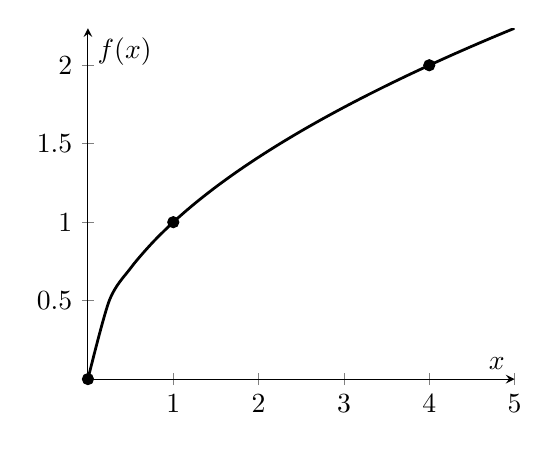
\begin{tikzpicture}
\begin{axis}[axis lines = center, xlabel = $x$, ylabel = {$f(x)$}]
\addplot[black, line width = 1, smooth, domain=-1:5] {sqrt(x)};
\addplot[mark=*] coordinates {(0,0) [$(0,0)$]};
\addplot[mark=*] coordinates {(1,1)};
\addplot[mark=*] coordinates {(4,2)};
\end{axis}
\end{tikzpicture}
\end{center}
\\
The negative values of $x$ and $y$ are not present since you cannot express imaginary numbers in a real number graph. This is why the graph is only shown at the first quadrant.
\subsection*{2.2 Square Root of a Function}
\\
When taking the square root of a function, $f(x)$, the invariant points will always be the x-intercepts (when $x=0$) and when $f(x)$ is 1. To graph it, take out the negative $f(x)$ values from the original and plot the invariant points. If the graph opens up, the square root function will go from $-\infty$ to $\infty$. Otherwise, the domain will be in-between the x-intercepts.

\section{Polynomial Functions}

\subsection*{3.1 Characteristics of Polynomial Functions}

A polynomial function has the form $f(x)=a_n x^n + a_{n-1} x^{n-1} + a_{n-2} x^{n-2} + ... + a_2x^2 + a_1x + a_0$, where $a_n$ is the leading coefficient; $a_0$ is the constant; and the degree of the polynomial, $n$, is the exonent of the greatest power of the variable, $x$. The number of x-intercepts can potentially have many as the function's highest degree. \\
\\
Odd-degree polynomial functions are graphs that extends down into quadrant III and up to quadrant I, which is similar to $y=x$ if the leading coefficient is positive. \\
\\
Even-degree polynomial functions are graphs that extends up to quadrant II and quadrant I, which is similar to $y=x^2$ if the leading coefficient is positive.

\subsection*{3.2 The Remainder Theorem}

Long division is a technique to find x-intercepts of a polynomial function that has a degree way above than 2.

\begin{tcolorbox}
	\textbf{Example}
	\begin{center}
		 \polylongdiv{-x^4-2x^3+7x^2+8x-12}{x-1}
	\end{center}
	\begin{equation*}
		f(x)=(x-1)(-x^3-3x^2+4x+12)
	\end{equation*}
\end{tcolorbox}

You can divide polynomials by other polynomials using the same long division process that you use to divide numbers. The result of the division of a polynomial in $x$, $P(x)$, by a binomial of the form $x - a, a\epsilon \mathbb{Z}$, is: \\

\begin{tcolorbox}
	\begin{equation*}
		\frac{P(x)}{x-a}= Q(x) + \frac{R}{x-a}
	\end{equation*}
$Q(x)$ = quotient \\
$x - a$ = binomial divisor \\
$R$ = remainder \\
$P(x)$ = polynomial dividend 
	\begin{equation*}
		P(x)=(x-a)Q(x)+R
	\end{equation*}
\end{tcolorbox}

Synthetic is also an alternative for long division, which is usually quicker and does not require you to write variables. It only involves the binomial divisor and only the coefficients of the terms.

\begin{tcolorbox}
	\textbf{Example}
	\begin{center}
		\polyhornerscheme[x=1]{-x^4-2x^3+7x^2+8x-12} 
	\end{center}
	\begin{equation*}
		f(x)=(x-1)(-x^3-3x^2+4x+12)
	\end{equation*}
\end{tcolorbox}

\subsection*{3.3 The Factor Theorem}

The factor theorem states that $x - a$ is a factor of a polynomial in $x$, $P(x)$, if and only if $P(a) = 0$. This means that if a binomial divisor is a factor of $P(x)$, then it would be equal to 0. Otherwise, it isn't a factor at all.

\begin{tcolorbox}
	\textbf{Example} Determine if $x-1$ and $x+2$ are factors of $P(x)=x^3-x^2-5x+2$.
	\begin{align*}
		P(1)&=(1)^3-(1)^2-5(1)+2 \\
		P(1)&= 1 - 1 - 5 + 2) \\
		P(1)&= -3 \\
		P(1)&\ne 0, \text{not a factor} \\
		\\
		P(-2)&=(-2)^3-(-2)^2-5(-2)+2 \\
		P(-2)&= -8 -4 + 10 + 2 \\
		P(-2)&= 0, \text{is a factor}
	\end{align*}
\end{tcolorbox}

The relationship between the factors of a polynomial and the constant term of the polynomial is stated in the integral zero theorem. \\
\\
The integral zero theorem states that if $x - a$ is a factor of a polynomial function $P(x)$ with integral coefficients, then $a$ is a factor of the constant term of $P(x)$. \\
\\
Descartes' rule of signs is helpful for finding the zeros of a polynomial. The way how it works is you ignore the coefficients and count the sign changes from left to right (positive to negative, or negative to positive). The number of sign changes you count is the maximum number of positive zeros for the polynomial. \\
\\
The rational root theorem is $\frac{p}{q}$, where $p$ is the constant and $q$ is the leading coefficient. This $\frac{p}{q}$ rational number is a root of the equation.

\begin{tcolorbox}
	\textbf{Example} Given $f(x)=2x^5+3x^4-6x^3+6x^2-8x+3$, demonstrate Descartes' rule of signs and the rational root theorem.
	\begin{equation*}
		\frac{p}{q}=\frac{3}{2}=\frac{\pm1,3}{\pm1,2}=\pm1, \pm3, \pm\frac{1}{2}, \pm\frac{3}{2} \leftarrow \text{All possible rational roots of $f(x)$}
	\end{equation*}
	
	\begin{center}
		$f(x) = + \rightarrow - \rightarrow + \rightarrow - \rightarrow +$
	\end{center}
	There are 4 possible positive roots of $f(x)$.
\end{tcolorbox}

A non-real root is when you take a square root of a negative number. If you have $\pm\sqrt{-9}$, you can simplify it to $\pm\sqrt{-1}*\sqrt{9}$ and $\sqrt{-1}$ can be written as $i$ as in imaginary. The imaginary number of this expression is $\pm3i$.

\subsection*{3.4 Equations and Graphs of Polynomial Functions}
Multiplicity is the number of times a zero of a polynomial function occurs. The shape of the graph of a function close to a zero depends on its multiplicity. If the multiplicity is 1, the graph goes through the zero once. If it's 2, it bounces of instead of going it through. If it's 3, the graph goes through, stays on the axis, then launches off (similar to an odd-degree function). \\
\\
Finding the first derivative of a polynomial function can help you find the local/global maximum/minimum point of the graph. You can do this by using the power rule formula $f'(x)=(an)x^{n-1}$ where $a$ is the coefficient, and $n$ is the degree of the variable, $x$. After that, set $f'(x)=0$ and find the roots, which then will be substituted in the original $f(x)$ equation.
\\
\\
\subsection*{Extra: Factoring Techniques}
\textbf{Case 1: Common Factoring}
	\begin{tcolorbox}
	\textbf{Example}
		\begin{align*}
			x^3-x^2-12x&=x(x^2-x-12) \\
			&=x(x-4)(x+3)
		\end{align*}
	\end{tcolorbox}
\textbf{Case 2: The Sum and Difference of Cubes}
	\begin{tcolorbox}
		\textbf{General Formula}
		\begin{center}
			$a^3x^3+d^3=(ax+d)(a^2x^2-adx+d^2)$
			$a^3x^3-d^3=(ax-d)(a^2x^2+adx+d^2)$
		\end{center}
		\textbf{Examples}
		\begin{align*}
			64x^3+125&=(4x+5)(16x^2-20x+25) \\
			\\
			3x^4 - 192x&=3x(x^3-64) \\
			&=3x(x-4)(x^2+4x+16)
		\end{align*}
	\end{tcolorbox}
\textbf{Case 3: Quartic Expressions Factored as Trinomials}
	\begin{tcolorbox}
		A quartic expression like $x^4-5x^2+4$ can be turned into $(x^2)^2-5x^2-4$ which factors as $(x^2-4)(x^2-1)$. Each of these factors can be further factored as the difference of two squares. \\
		\\
		\textbf{Example}
		\begin{align*}
			4x^4-37x^2+9&=(x^2-9)(4x^2-1) \\
			&=(x-3)(x+3)(2x-1)(2x+1)
		\end{align*}
	\end{tcolorbox}
\\
\textbf{Case 4: Grouping to Find a Common Factor}
\begin{tcolorbox}
	\textbf{Example}
	\begin{align*}
		&8x^5-40x^4+32x^3-x^2+5x-4 \\
		&=8x^3(x^2-5x+4)-(x^2-5x+4) \\
		&=(8x^3-1)(x^2-5x+4) \\
		&=(4x^2+2x+1)(2x-1)(x-4)(x-1)
	\end{align*}
\end{tcolorbox}

\textbf{Case 5: Grouping to Get the Difference of Squares}
\begin{tcolorbox}
	\textbf{Example}
	\begin{align*}
		x^4-6x^2+1&=x^4-2x^2+1-4x^2 \\
		&=(x^2-1)^2-4x^2 \\
		&=(x^2-1-2x)(x^2-1+2x)
	\end{align*}
\end{tcolorbox}

\section{Trigonometry}
\begin{center}
	$f(x)=sin(x)$
	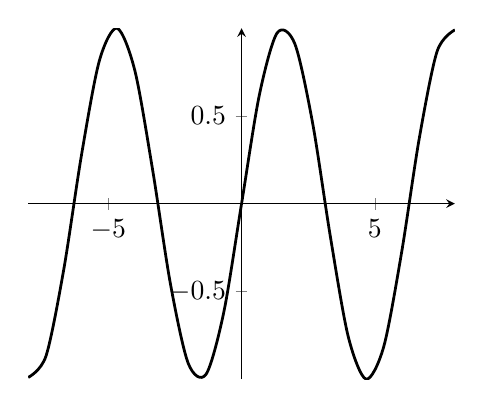
\begin{tikzpicture}
		\begin{axis}[axis lines = center]
			\addplot[black, line width = 1, smooth, domain=-8:8] {sin(deg(x))};
		\end{axis}
	\end{tikzpicture}
\end{center}

\begin{center}
	$g(x)=cos(x)$
	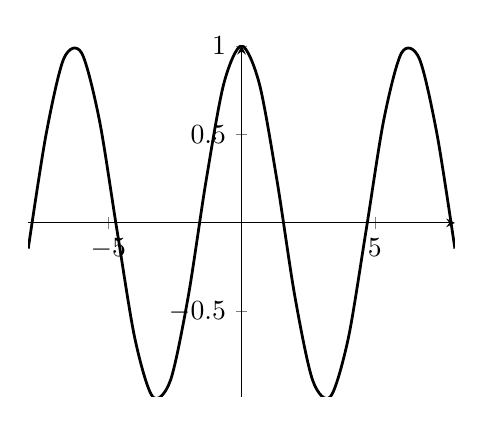
\begin{tikzpicture}
		\begin{axis}[axis lines = center]
			\addplot[black, line width = 1, smooth, domain=-8:8] {cos(deg(x))};
		\end{axis}
	\end{tikzpicture}
\end{center}

\subsection{Transformations of Sinusodial Equations}

\begin{tcolorbox}
	\begin{center}
		$f(x)=asin[b(x-h)] + k$ or $f(x)=acos[b(x-h)] + k$
	\end{center}
	$a$ = Vertical Stretch/Reflection on the x-axis or Amplitude \\
	$b$ = Horizontal Stretch or Period \\
	$h$ = First place on the SA (for sine) or First maximum point (for cosine) \\
	$k$ = Vertical Translation or the Sinusodial Axis (also known as the horizontal asymptote)
\end{tcolorbox}

\section{Rational Functions}
\subsection{Graphing Rational Functions}
\textbf{Step 1}
\begin{itemize}
	\item Factor
	\item Points of Discontinuity occurs when factors cancel
\end{itemize}
\textbf{Step 2}
\begin{itemize}
	\item Identify intercepts
	\subitem x-intercepts occur at the numerator
	\subitem y-intercept occurs when $x=0$
\end{itemize}
\textbf{Step 3}
\begin{itemize}
	\item Vertical Asymptotes occurs at the denominator
	\item Horizontal Asymptotes
	\subitem n $<$ d $\rightarrow$ $y=0$
	\subitem n = d $\rightarrow$ $\div$ leading coefficients
	\subitem n $>$ d $\rightarrow$ O.A.
	\item Oblique Asymptotes
	\subitem When n $>$ d, use long division to find the oblique asymptote, which is a linear equation like $y=x$.
\end{itemize}

\textbf{Crossing the H.A. or O.A.}
\begin{itemize}
	\item Set H.A. or O.A. equal to $f(x)$
	\subitem $ 1 = \frac{x^2+x-12}{x^2-4} $
	\item If $x$ values do not cancel out but gives you an $f(x)$ value, that means it does cross through the said asymptote.
\end{itemize}
\end{document}
